% ============================================================
%  CHAPTER 6 — Experimental Results and Analysis
% ============================================================

\chapter{Experimental Results and Analysis}
\label{ch:results}

This chapter reports the measured performance of the trained controllers. All
values are computed by the evaluation pipeline described in
\cref{chap:impl} and read from the run artifacts named beneath each table;
none is hand-entered.

\section{Evaluation metrics}

Two distance measures are reported throughout, because they capture different
failure modes. \emph{Final error} is the hand--target distance at the end of the
two-second reach; \emph{closest approach} is the smallest distance attained at
any instant. Their difference, the \emph{drift}, quantifies how far the hand
wanders back out after arriving.

A controller that sweeps through the target at speed scores well on closest
approach and badly on final error. Separating the two proved essential: it
revealed that the task presented two independent difficulties, with different
causes and different remedies.

\begin{table}[H]
\centering
\caption{Metrics used in this chapter.}
\begin{tabular}{@{} L{4.0cm} L{9.0cm} @{}}
\toprule
\textbf{Metric} & \textbf{Definition} \\
\midrule
Final error & hand--target distance at end of episode \\
Closest approach & minimum hand--target distance during the episode \\
Drift & final error minus closest approach \\
Reach 5/10\,cm & fraction of episodes \emph{ending} within that distance \\
Touch 2/5\,cm & fraction of episodes attaining that distance at any instant \\
Energy & $\sum_i F_i^2$, a metabolic-cost proxy \\
Blow-up rate & fraction of episodes ending in numerical divergence \\
\bottomrule
\end{tabular}
\label{tab:metrics}
\end{table}

\subsection{The reference bound}

To interpret any of these numbers, an achievable bound is required. A privileged
controller, granted information the learned policy does not receive, attains a
median final error of \SI{0.08}{\meter} and comes within \SI{2}{\centi\meter} at
some instant in 27\,\% of episodes. Under the strict success criterion --- within
\SI{2}{\centi\meter} \emph{and} nearly stationary --- it succeeds approximately
7\,\% of the time.

This bound has a direct methodological consequence. A criterion that a
near-best-possible controller satisfies only 7\,\% of the time cannot discriminate
among learned policies, and \textbf{success rate is therefore not used as a
headline metric in this work}. Graded measures are reported instead.

\section{Effect of correcting the replay ratio}
\label{sec:replayresult}

\Cref{sec:replaybug} identified that training had been performing approximately
one quarter of its intended gradient updates. Correcting this, with no other
change, produced the comparison in \cref{tab:replay}.

\begin{table}[H]
\centering
\caption{Effect of the replay-ratio correction. Identical reward, model, seed
and evaluation protocol; the corrected run uses \emph{fewer} environment steps.}
\begin{tabular}{@{} L{5.4cm} C{3.2cm} C{3.2cm} @{}}
\toprule
\textbf{Metric} & \textbf{Ratio 0.23} & \textbf{Ratio 0.93} \\
\midrule
Environment steps & 1\,000\,000 & 300\,000 \\
Final error (m) & 0.254 & \textbf{0.204} \\
Closest approach (m) & 0.134 & 0.132 \\
Drift (m) & 0.120 & \textbf{0.072} \\
Energy & $1.25\times10^{6}$ & \textbf{$0.77\times10^{6}$} \\
Blow-up rate & 2\,\% & \textbf{0\,\%} \\
Path length per \SI{0.80}{\meter} reach (m) & 3.76 & 3.55 \\
\bottomrule
\end{tabular}
\label{tab:replay}
\end{table}

The correction improved \emph{holding} substantially --- drift nearly halved,
divergences eliminated, energy reduced by 38\,\% --- while \emph{closest
approach} was unchanged, moving only from \SI{0.134}{} to \SI{0.132}{\meter}.

That immobility is informative. Closest approach had remained near
\SI{0.13}{\meter} across three complete redesigns of the reward function and this
fourfold increase in effective training. Its insensitivity to both indicated that
the residual limitation lay elsewhere, and motivated the hyperparameter study of
\cref{sec:tuning}.

\section{Hyperparameter optimisation}
\label{sec:tuning}

A sixteen-trial Bayesian optimisation (Optuna, TPE sampler with median pruning)
was performed over learning rate, discount factor, batch size, target-network
update rate and target entropy. Thirteen trials completed; three were pruned.

\begin{table}[H]
\centering
\caption{Five best trials, ranked by final error at 100\,000 steps.}
\begin{tabular}{@{} C{1.6cm} C{2.4cm} C{2.8cm} C{2.8cm} C{2.2cm} @{}}
\toprule
\textbf{Trial} & \textbf{Final error} & \textbf{Learning rate} & \textbf{Target entropy} & \textbf{Drift} \\
\midrule
12 & \textbf{0.1177} & $4.40\times10^{-4}$ & $-19.6$ & 0.034 \\
14 & 0.1293 & $3.91\times10^{-4}$ & $-20.0$ & 0.051 \\
11 & 0.1311 & $4.22\times10^{-4}$ & $-19.3$ & 0.049 \\
13 & 0.1405 & $4.38\times10^{-4}$ & $-18.6$ & 0.069 \\
10 & 0.1405 & $4.49\times10^{-4}$ & $-19.0$ & 0.035 \\
\bottomrule
\end{tabular}
\label{tab:optuna}
\end{table}

Every one of the five best trials selects a target entropy close to $-19$,
against the \SAC default of $-\dim(\mathcal{A}) = -9$ for a nine-dimensional
action space. The search converges on a policy roughly twice as deterministic as
the standard heuristic prescribes.

The optimiser varied five parameters at once, however, and the target entropy was
not the only one to move appreciably: the target-network update rate $\tau$ rose
from 0.005 to 0.0188, a factor of 3.8, and the learning rate by 47\,\%. The
clustering of the best trials is suggestive but not decisive, since a TPE sampler
exploits promising regions and will cluster whether or not the clustered
parameter is the causal one. Attribution to the target entropy specifically is
therefore advanced here as the leading hypothesis --- its mechanism matches the
symptom, an inability to settle --- and not as an established result. The
one-at-a-time ablation that would settle it is set out in \cref{sec:future}.

The target entropy governs how much stochasticity \SAC deliberately retains in
its policy. Exploration is valuable early in training, but must diminish for the
end effector to settle precisely. The optimiser's consistent preference for a
substantially lower value indicates that the default maintains more residual
noise in the commanded activations than this task tolerates.

\subsection{Confirmation at full budget}
\label{sec:confirmresult}

The selected hyperparameters were retrained from initialisation under the full
300\,000-step protocol with fifty-episode evaluation, to verify that the result
was not an artefact of the search's reduced budget.

\begin{table}[H]
\centering
\caption{Confirmation run against the previous configuration. Both are \SAC,
seed 0, 300\,000 steps, fifty evaluation episodes, differing only in
hyperparameters.}
\begin{tabular}{@{} L{5.6cm} C{3.0cm} C{3.0cm} @{}}
\toprule
\textbf{Metric} & \textbf{Default hyperparameters} & \textbf{Tuned hyperparameters} \\
\midrule
Final error (m) & 0.204 & \textbf{0.106} \\
Closest approach (m) & 0.132 & \textbf{0.074} \\
Drift (m) & 0.072 & \textbf{0.035} \\
Ends within \SI{5}{\centi\meter} & 0\,\% & \textbf{34\,\%} \\
Ends within \SI{10}{\centi\meter} & 18\,\% & \textbf{58\,\%} \\
Attains \SI{2}{\centi\meter} at any instant & 2\,\% & \textbf{20--28\,\%} \\
Energy & 774\,667 & \textbf{276\,804} \\
Path length per \SI{0.80}{\meter} reach (m) & 3.55 & \textbf{1.64} \\
Success rate & 0\,\% & 4\,\% \\
\bottomrule
\end{tabular}
\label{tab:confirm}
\end{table}

Closest approach improved from \SI{0.132}{} to \SI{0.074}{\meter}, below the
privileged controller's median final error of \SI{0.08}{\meter}. The proportion
of episodes attaining \SI{2}{\centi\meter} reached 28\,\%, comparable to the
privileged controller's 27\,\%: a policy acting on proprioceptive information
alone approached the performance of one with full state access.

Path length fell from \SI{3.55}{} to \SI{1.64}{\meter} for the same
\SI{0.80}{\meter} of required travel, with net displacement $0.99\times$ the
distance required. The end effector ceased sweeping through the target region and
began travelling to it directly.

Two qualifications apply to \cref{tab:confirm}. The success rate of 4\,\%
corresponds to two episodes in fifty; an independent re-evaluation over a
different set of fifty targets returned 2\,\%, that is one episode. At this
magnitude the metric is dominated by sampling noise and should not be interpreted
as a performance level. Secondly, the table reports a single training seed;
replication across seeds remains outstanding.

\begin{figure}[H]
\centering
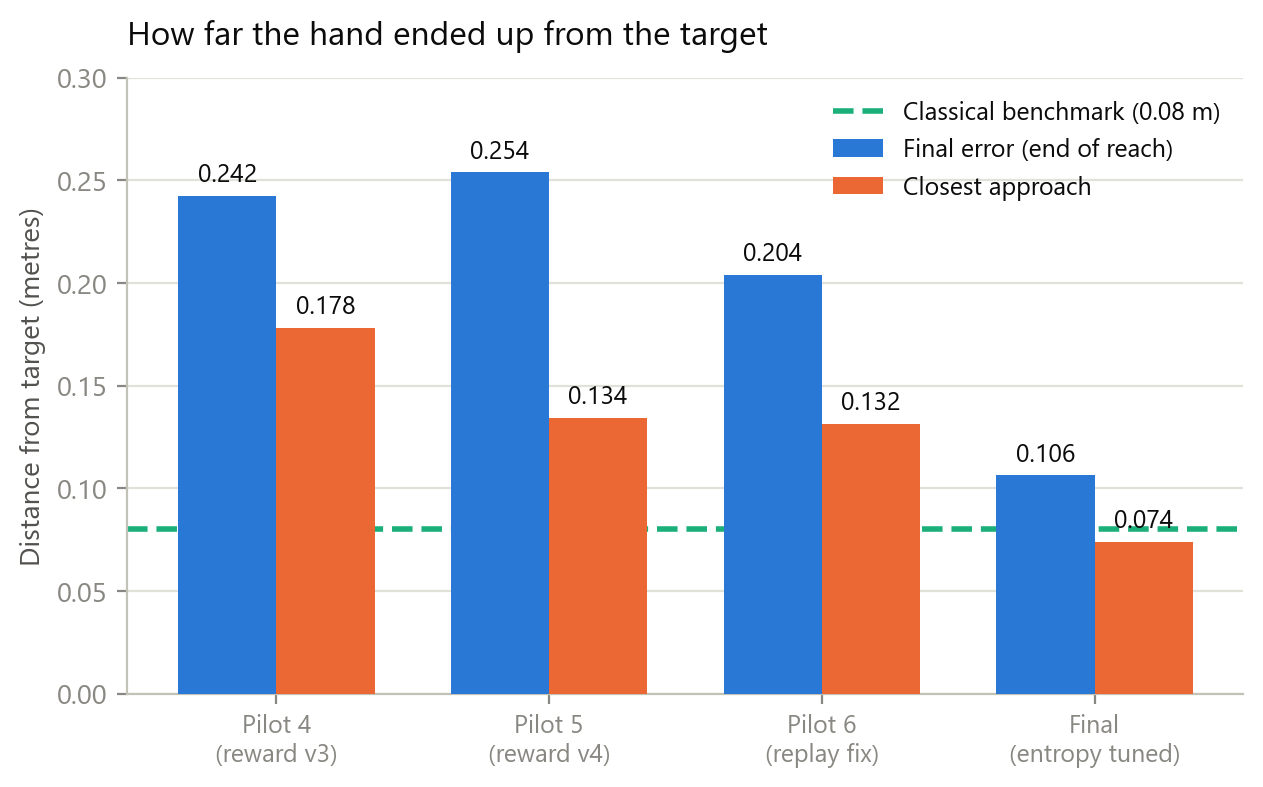
\includegraphics[width=0.92\textwidth]{figures/fig1_progression.png}
\caption{Reaching error across the four principal experiments. Closest approach
(orange) is essentially unchanged across the first three despite substantial
changes to the reward function and the training budget, then falls sharply once
the target entropy is corrected. The dashed line marks the privileged
controller's median final error.}
\label{fig:progression}
\end{figure}

\subsection{Intra-episode behaviour}

\begin{table}[H]
\centering
\caption{Mean hand--target distance during a reach, averaged over thirty
episodes.}
\begin{tabular}{@{} C{2.6cm} C{3.4cm} C{3.4cm} @{}}
\toprule
\textbf{Step} & \textbf{Default entropy} & \textbf{Tuned entropy} \\
\midrule
0  & 0.795 & 0.795 \\
10 & 0.314 & 0.198 \\
25 & 0.203 & 0.119 \\
50 & 0.184 & 0.110 \\
75 & 0.184 & 0.112 \\
99 & 0.177 & \textbf{0.113} \\
\bottomrule
\end{tabular}
\label{tab:traj}
\end{table}

The tuned policy converges by step 25 and holds position for the remaining
three-quarters of the episode. Target tracking is strong, with correlations of
0.94, 0.90 and 0.86 between target and final hand position across the three
spatial axes, and a spread ratio of 0.91.

\begin{figure}[H]
\centering
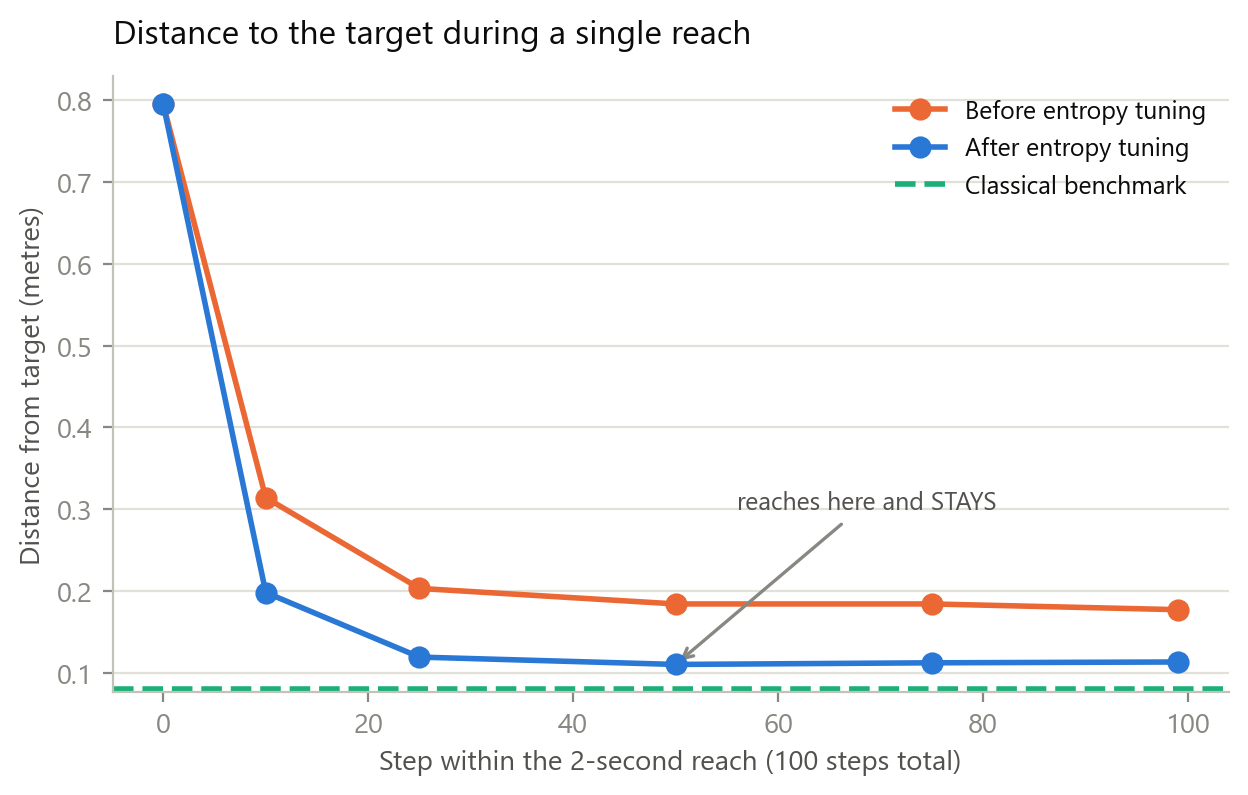
\includegraphics[width=0.92\textwidth]{figures/fig2_trajectory.png}
\caption{Hand--target distance during a single two-second reach, averaged over
thirty episodes. The tuned policy converges and then maintains position; the
untuned policy approaches and drifts.}
\label{fig:trajectory}
\end{figure}

\section{Algorithm comparison}
\label{sec:benchmark}

Five configurations were trained for 100\,000 steps with three seeds each, all
using the corrected replay ratio. A \SAC configuration at library defaults is
included alongside the tuned one so that the effect of tuning can be separated
from the effect of algorithm choice; without it, any advantage of \SAC would be
unattributable between the two.

\begin{table}[H]
\centering
\caption{Algorithm comparison: five configurations, three seeds each,
100\,000 steps. Mean $\pm$ standard deviation across seeds.}
\small
\begin{tabular}{@{} L{2.7cm} C{2.6cm} C{2.6cm} C{1.7cm} C{1.9cm} C{1.5cm} @{}}
\toprule
\textbf{Configuration} & \textbf{Final error (m)} & \textbf{Closest (m)} & \textbf{Ends $<$10\,cm} & \textbf{Energy} & \textbf{Minutes} \\
\midrule
\SAC tuned   & $\mathbf{0.161 \pm 0.008}$ & $\mathbf{0.093 \pm 0.009}$ & \textbf{0.37} & 597\,k & 30 \\
\SAC default & $0.261 \pm 0.020$ & $0.129 \pm 0.004$ & 0.05 & 1187\,k & 46 \\
\TDIII       & $0.279 \pm 0.011$ & $0.165 \pm 0.017$ & 0.10 & 1242\,k & 21 \\
\DDPG        & $0.416 \pm 0.019$ & $0.218 \pm 0.026$ & 0.03 & 1384\,k & 23 \\
\PPO         & $0.423 \pm 0.035$ & $0.238 \pm 0.071$ & 0.05 & 202\,k & 3 \\
\bottomrule
\end{tabular}
\label{tab:benchmark}
\end{table}

\begin{figure}[H]
\centering
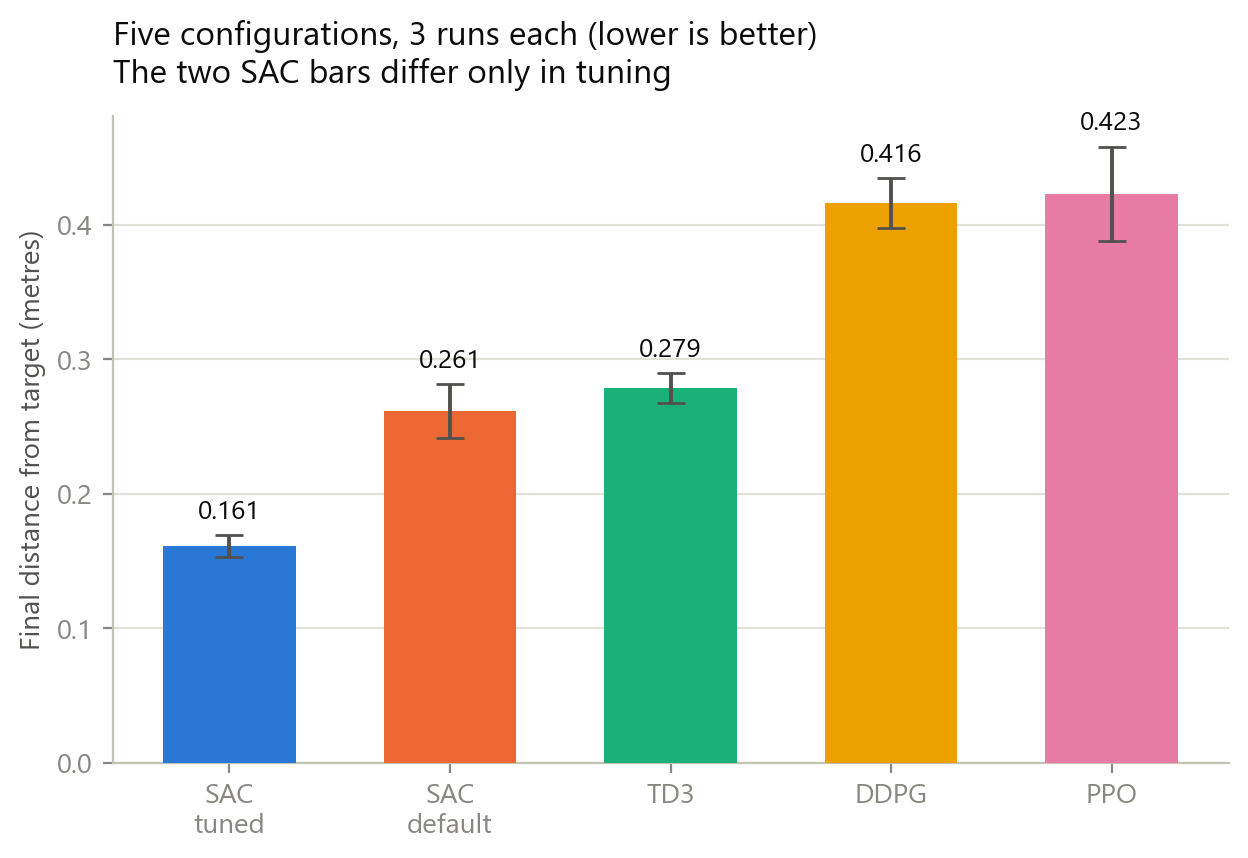
\includegraphics[width=0.92\textwidth]{figures/fig3_benchmark.png}
\caption{Final reaching error by configuration; error bars are one standard
deviation across three seeds. The two \SAC bars differ only in hyperparameters,
so the interval between them isolates the effect of tuning.}
\label{fig:benchmark}
\end{figure}

Tuning \SAC reduced final error from 0.261 to \SI{0.161}{\meter}, an improvement
of 38\,\%. The interval between untuned \SAC and \TDIII is 0.261 against 0.279,
approximately 6\,\%, against seed standard deviations of 0.020 and 0.011; this
difference is comparable to the spread and does not support an ordering. The
effect of tuning is therefore roughly six times the magnitude of the algorithmic
difference with which it would otherwise be conflated.

\DDPG and \PPO are both substantially worse than \TDIII, by approximately
\SI{0.14}{\meter} --- many times the seed spread. For \DDPG this is consistent
with the theoretical expectation of \cref{chap:drl}, as it lacks the twin
critics that mitigate value overestimation. \DDPG and \PPO are, however,
indistinguishable from one another.

Three constraints limit what this comparison establishes. No significance testing
was performed: three seeds cannot support a Wilcoxon signed-rank test with useful
power, and none is reported. The comparison is an early-training snapshot at
100\,000 steps, whereas the best configuration attains \SI{0.106}{\meter} at
300\,000 steps (\cref{tab:confirm}), so orderings may change with budget. And
\TDIII, \DDPG and \PPO were run at library defaults while \SAC received a
sixteen-trial search, so any comparison involving the tuned configuration
conflates algorithm with tuning effort by construction. Success rate is 0\,\% for
every configuration at this budget and is omitted for that reason.

\subsection{Interpretation of the PPO result}

\PPO's position requires care. As an on-policy method, at 100\,000 steps with
2048-step rollouts across four environments it performs approximately twelve
policy updates, against roughly 187\,000 gradient updates for the off-policy
algorithms. It also completes in three minutes against 21--46 for the others.
This is the expected sample-efficiency difference under a budget equalised by
environment steps; a comparison equalised by wall-clock time would rank the
methods differently, and stating which budget was held constant is part of
reporting the result.

Its energy consumption is also distinctive: 202\,k against 597\,k for tuned \SAC
and 1187--1384\,k for the remainder, between three and seven times lower.
Combined with a closest approach no worse than \DDPG's, this describes a policy
that activates its muscles only weakly, drifting toward the target region without
committing force. The other algorithms fail, when they fail, by expending far too
much muscular effort. These are opposite failure modes, and a single accuracy
figure conceals the distinction entirely --- a point developed in
\cref{ch:forces}.

Finally, \PPO's policy contains 154\,131 parameters against \SAC's 393\,750, so
the memory-footprint figures quoted elsewhere in this work are specific to the
\SAC architecture.

\section{Computational efficiency}
\label{sec:compute_efficiency}

The motivation for a learned controller is inference cost. Both methods were
timed on the same host processor over 950 queries.

\begin{table}[H]
\centering
\caption{Inference cost: iterative Newton--Raphson solution against a single
forward pass of the trained network.}
\begin{tabular}{@{} L{6.4cm} C{3.2cm} C{3.2cm} @{}}
\toprule
\textbf{Quantity} & \textbf{Newton--Raphson} & \textbf{Network} \\
\midrule
Mean latency & \SI{2165}{\micro\second} & \SI{295}{\micro\second} \\
Standard deviation & \SI{319}{\micro\second} & \SI{45}{\micro\second} \\
95th percentile & \SI{2657}{\micro\second} & \SI{364}{\micro\second} \\
99th percentile & \SI{2897}{\micro\second} & \SI{480}{\micro\second} \\
Mean iterations & 31.2 & 1 (fixed) \\
\bottomrule
\end{tabular}
\label{tab:nr_vs_rl}
\end{table}

The mean speed-up over the Newton--Raphson solver is $7.3\times$, and the
network's cost is fixed where the iterative solver's is data-dependent.

\subsection{This comparison does not support a deployment claim}
\label{sec:latencycaveat}

Two objections apply to \cref{tab:nr_vs_rl}, and together they are decisive.

\textbf{It times the wrong computation.} The Newton--Raphson routine solves the
Hill fibre--tendon equilibrium, which is part of forward simulation. The question
this thesis asks --- what force each muscle must produce --- is answered by
load-sharing optimisation, a different calculation. The two have been conflated.

\textbf{Both sides were unoptimised Python.} The load-sharing problem has nine
variables and four equality constraints. Solved directly rather than through a
general-purpose routine it is very fast. Measured on an idle machine, one torch
thread, 400 queries:

\begin{table}[H]
\centering
\caption{Load-sharing latency, measured like-for-like. Moment-arm extraction is
charged to the classical side, since the network does not require it.}
\begin{tabular}{@{} L{7.2cm} R{2.0cm} R{2.0cm} R{2.0cm} @{}}
\toprule
\textbf{Method} & \textbf{mean} & \textbf{p95} & \textbf{p99} \\
\midrule
Network forward pass & 288.8 & 332.6 & 499.9 \\
Classical, general solver (SLSQP) & 2370.5 & 4023.7 & 5133.1 \\
Classical, direct solve $+$ moment arms & \textbf{23.9} & --- & --- \\
\bottomrule
\end{tabular}
\label{tab:loadsharing_latency}
\end{table}

Against a general-purpose solver the network is $8.2\times$ faster. Against a
direct solve of the same problem it is \textbf{approximately twelve times
slower}.

\textbf{The latency argument for replacing classical calculation is therefore
withdrawn.} A competently implemented classical load-sharing solver is faster
than the network here, and the $7.3\times$ figure reflects the cost of one Python
implementation rather than a property of the two approaches.

A qualification in the other direction: the box constraints are active in
100\,\% of sampled states, so the closed-form solution timed above is not exactly
valid, and a constrained active-set solver would cost more than
\SI{23.9}{\micro\second}. It would not cost \SI{2370}{\micro\second}. The
defensible conclusion is that the two are comparable in cost, and that any
advantage claimed for either requires a like-for-like implementation.

What survives is the \emph{shape} of the cost rather than its magnitude: the
network's runtime is fixed and branch-free irrespective of biomechanical state,
whereas the iterative solver's depends on convergence. Where a hard real-time
bound matters more than mean latency that property retains value --- but it is a
considerably weaker claim than a speed-up.

The trained \SAC policy contains 393\,750 parameters, occupying
\SI{1.5}{\mega\byte} in single precision or \SI{385}{\kilo\byte} quantised to
eight bits. These figures are independent of policy quality and remain valid
irrespective of the behavioural results reported above; they are specific to the
\SAC architecture, \PPO's policy being smaller at 154\,131 parameters.
